%==============================================================================
\section{Grassroots Platforms and Resources}\label{section:platforms}
%==============================================================================

A grassroots platform operates solely on the smartphones of its members, forsaking any global resources other than the network itself.  Any group of people may initiate an instance of any grassroots platform, which may operate independently or coalesce with other instances of the platform into ever larger ones, possibly culminating in a global instance~\cite{shapiro2023grassrootsBA,shapiro2024grassroots,shapiro2025atomic,shapiro2025characterising,lewis2026volitional}.

\begin{figure}[h]
\centering
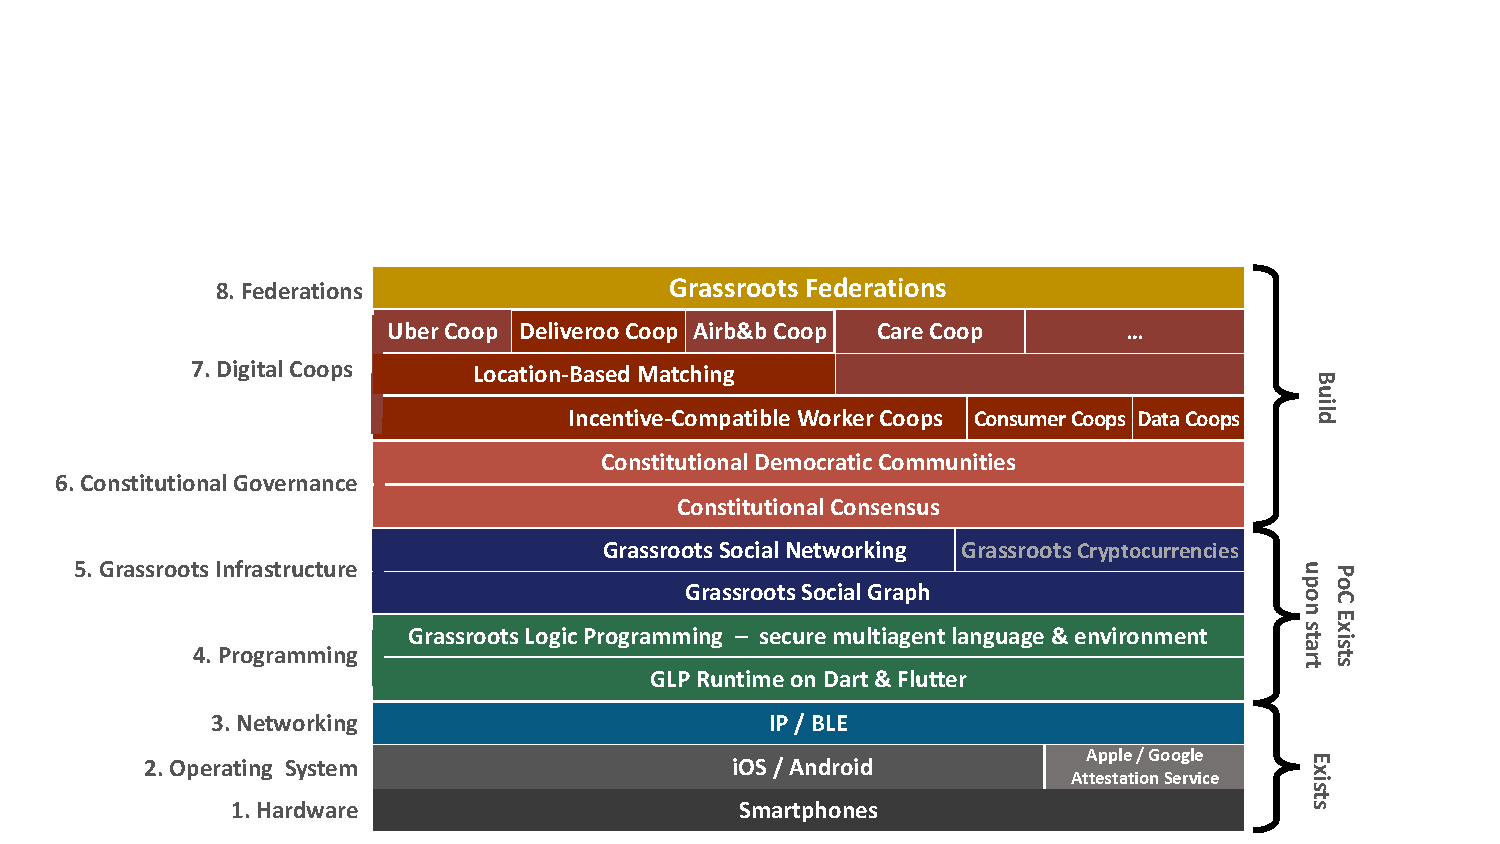
\includegraphics[width=\textwidth, trim=0 0 0 120, clip]{grassroots-stack-v12.pdf}
\caption{The grassroots protocol stack. GLP and its runtime constitute layer~4.}
\label{fig:stack}
\end{figure}

\mypara{Grassroots platforms specified and proven grassroots}
Concise specifications of the following grassroots platforms have been provided and proven grassroots: the grassroots social graph~\cite{shapiro2023gsn,shapiro2025atomic,lewis2026volitional}---the infrastructure platform on which all other grassroots platforms build, defined and implemented in this paper; grassroots social networks~\cite{shapiro2023gsn}, including private and public feeds, replies, reposts, mentions, follows, and groups; child-safe grassroots social networks~\cite{shapiro2026cssn}, with formally proved child-safety guarantees; grassroots cryptocurrencies~\cite{shapiro2024gc,lewis2023grassroots}, without consensus, mining, or globally-replicated state; grassroots bonds~\cite{shapiro2026bonds}, instruments for cooperative finance built on grassroots cryptocurrencies; and grassroots federations~\cite{shapiro2025GF,halpern2024federated}, sortition-based federations of sovereign communities with persistently-fair representation. The unifying formal framework for these specifications is volitional multiagent atomic transactions~\cite{lewis2026volitional}. GLP implementations of grassroots platforms --- the social graph (this paper), child-safe social networks~\cite{shapiro2026cssn}, and grassroots cryptocurrencies and bonds~\cite{shapiro2026bonds} --- are derived by AI from these specifications, with the child-safe social network exercised on a 6-agent village scenario and with child-safety, grassroots, liveness, and implementation correctness all formally proved~\cite{shapiro2026cssn}.

\mypara{Constitutional democratic governance}
Constitutional governance of grassroots communities and federations builds on Constitutional Consensus~\cite{keidar2025constitutional,lewis2025morpheus} and digital social contracts~\cite{cardelli2020digital,shapiro2022foundations}, both realisable in GLP.

\mypara{Companion GLP papers}
A companion paper~\cite{shapiro2026implementing} derives a deterministic implementation madGLP from maGLP, proves it grassroots, and presents the Dart/Flutter runtime. Another companion~\cite{shapiro2026types} develops moded types for GLP, supporting AI-assisted derivation of typed programs from specifications. A textbook on GLP and programming in it is in preparation.

\mypara{Source code}
The GLP runtime and example programs are open-source at \url{https://github.com/EShapiro2/GLP}.
